\section{\systemname Formalism}\label{sec:formal}

% \begin{itemize}
% \item Describe the types for checked-C as a graph. \dvh{I don't know what this means.}

% \item Describe the subtyping for checked-C types.
% \begin{itemize}
% \item State that the subtypes in Checked-C are transitive.
% \end{itemize}

% \item Describe the syntax of Checked-C

% \item Describe the semantics of Checked-C

% \item Describe the type system of Checked-C

% \item Describe the progress and preservation theorems, and outline the proofs.

% \item Describe the blame theorem and proof.

% \end{itemize}

% \ignore{
% \begin{figure}
%   \begin{center}
%     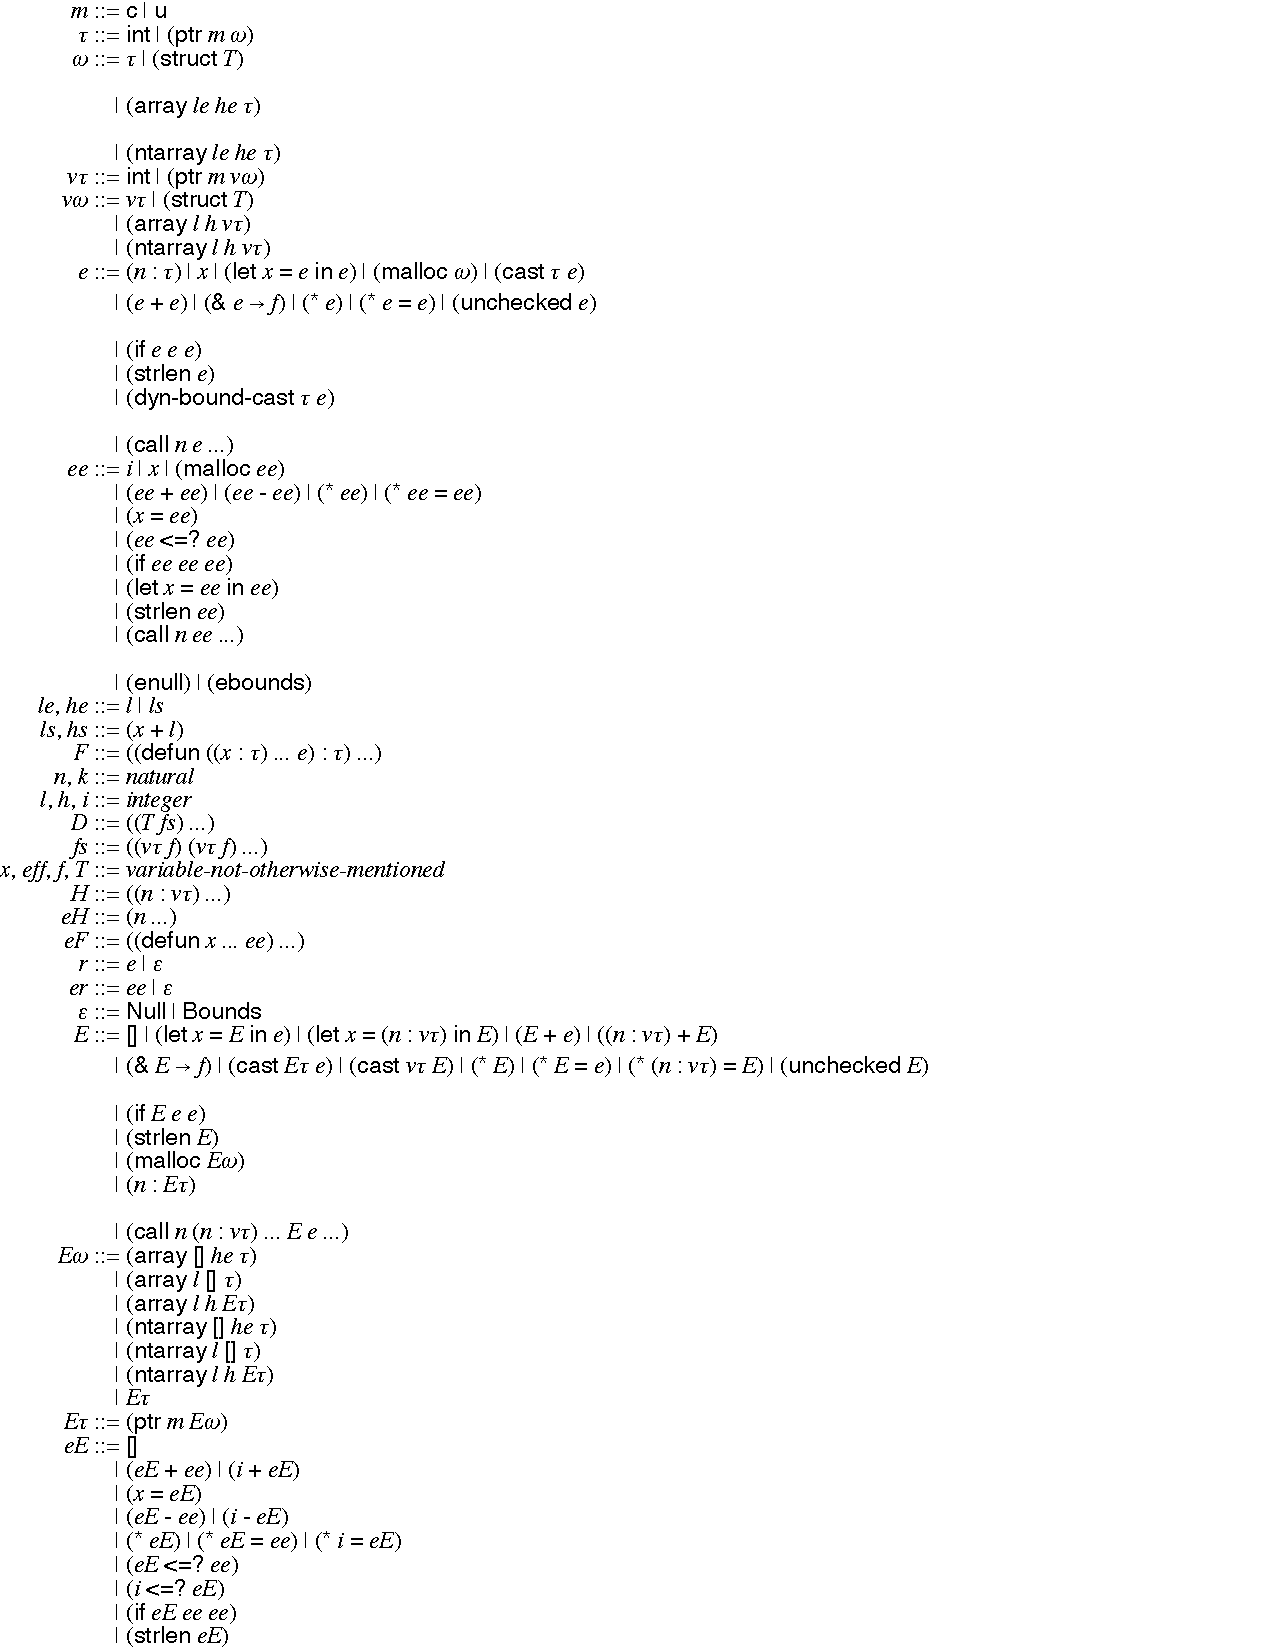
\includegraphics[height=6in]{syntax.pdf}
%   \end{center}
%   \caption{\lang: Syntax}
% \end{figure}

% \begin{figure}
%   \begin{center}
%     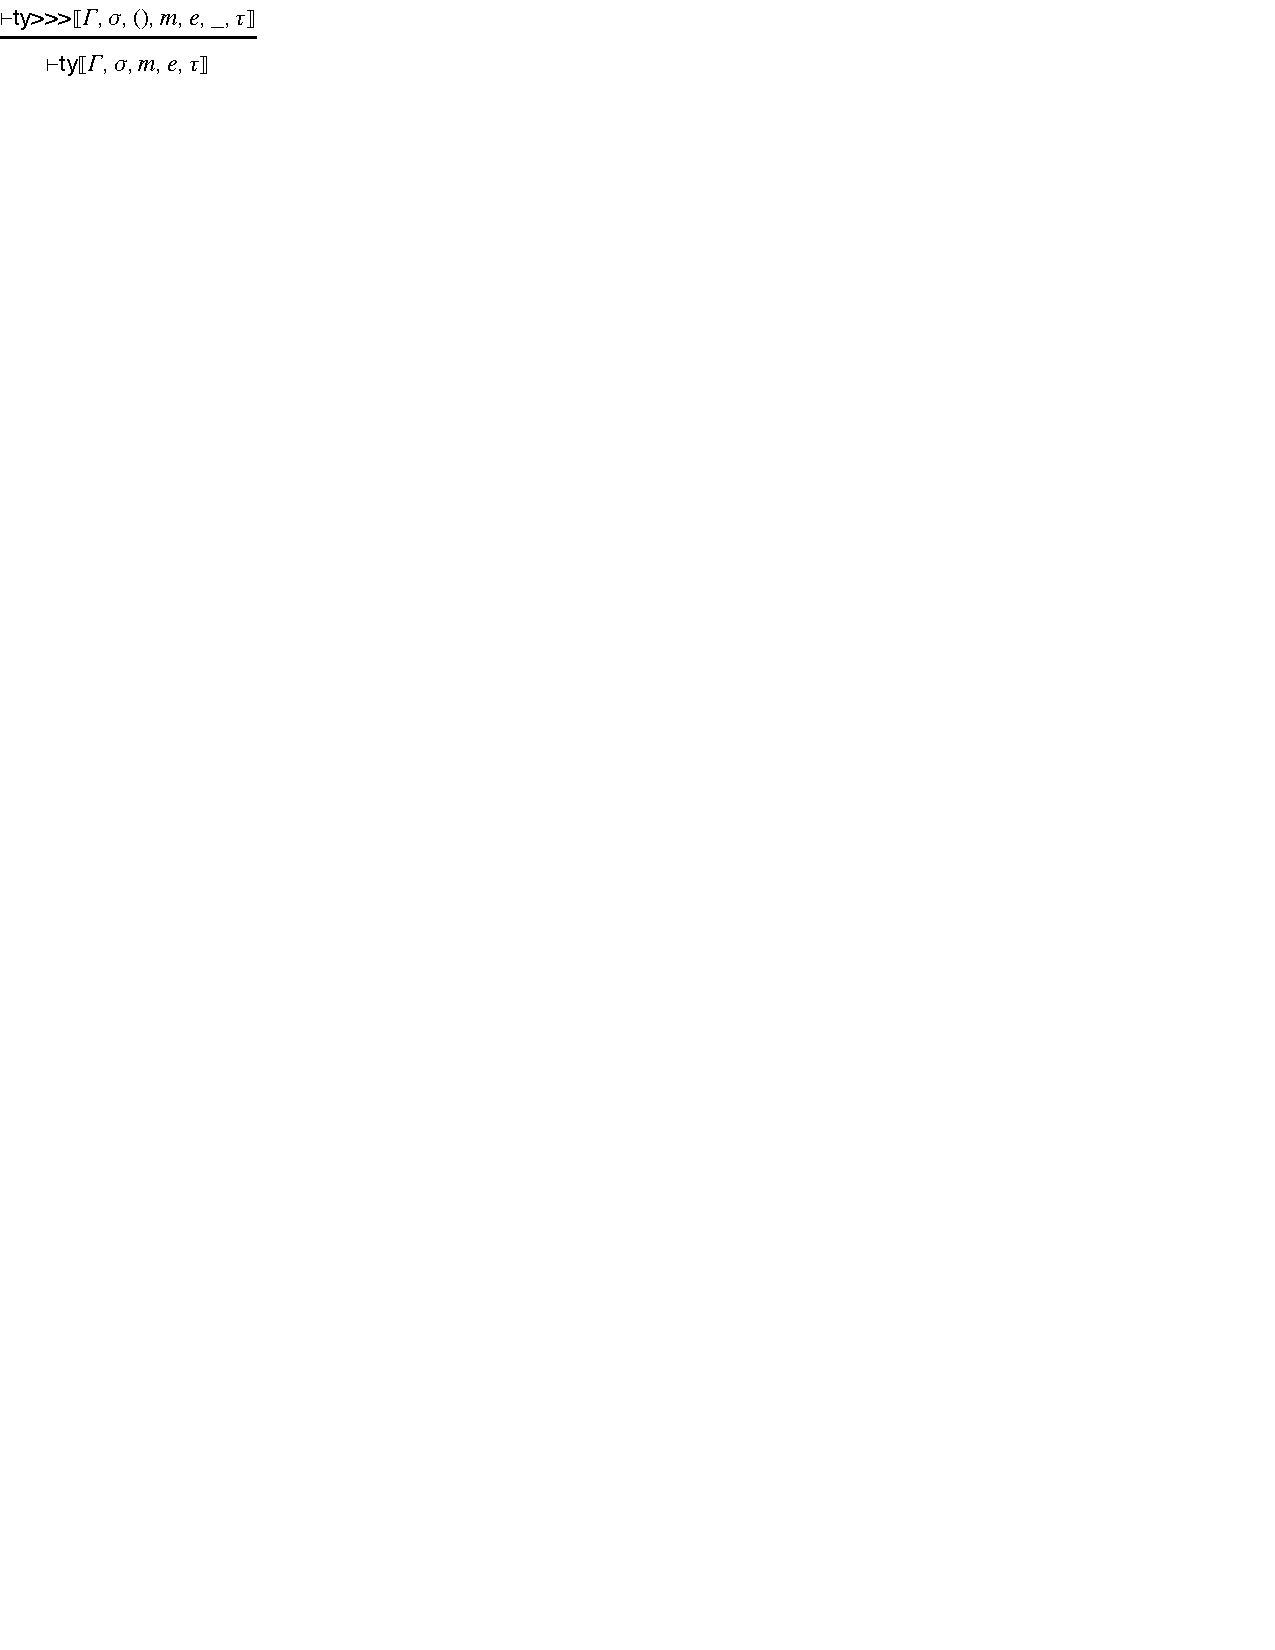
\includegraphics[height=6in]{types.pdf}
%   \end{center}
%   \caption{\lang: Typing}
% \end{figure}
% }
% \liyi{main text begins here. }

% \review{
% While reading the semantics, I found the fact that S-Def and S-DefNull are
%   applicable non-deterministically if n is 0 a bit confusing. Only when
%   reading the meta-theory section I realized that this is not a concrete issue
%   because well-formed heaps are such that $\mathcal{H}(0)$ is never defined. It
%   might be worth pointing this out early on. }
% \mwh{Done.}

\begin{figure}
  \small \centering
  \[ \hspace*{-1.2em}
\begin{array}{l}
\begin{array}{ll}
       \text{Variables:}~ x
& \text{Integers:}~n::=\mathbb{Z} 
\end{array}
\\[0.5em]
\begin{array}{llcllcl}
\text{Context Mode:} & m & ::= & \cmode \mid \umode \\
\text{Pointer Mode:} & \xi & ::= & m \mid \tmode \\
\text{Bound:} & b & ::= & n \mid x \plus n \\
              & \bvar & ::= & (b,b) \\
  
     \text{Word Type:}& \tau &::=& \tint\mid \tptr{\omega}{ \xi}
\\
\text{Type Flag:}&\kappa &::=& nt \mid \cdot
\\
\text{Type:}&\omega &::=& \tau \mid \tallarrayb{\bvar}{\tau} \mid \tfun{\overline{x}}{\overline{\tau}}{\tau}
\\
\text{Expression:}& e & ::= & 
\evalue{n}{\tau} \mid x \mid \ebinop{e}{e}\mid \ecast{\tau}{e} \mid \edyncast{\tau}{e}  \\
&&\mid& \estrlen{x} \mid \emalloc{\xi}{\omega} \mid\estar{e}\mid\eassign{e}{e}  \\
&&\mid& \elet{x}{e}{e} \mid \eif{e}{e}{e} \mid \ecall{e}{\overline{e}}
\\
&&\mid&\eunchecked{\overline{x}}{e}
\mid \echecked{\overline{x}}{e}
\end{array}
    \end{array}
  \]
  \caption{\lang Syntax}
  \label{fig:checkc-syn}
\end{figure}

\ignore{
\begin{figure}[t]
{\small
  \begin{mathpar}

  \inferrule[]
  {}
  {m \vdash \tint}

  \inferrule[]
  {\xi \wedge m\vdash \tau \\ \xi \le m}
  {m \vdash \tptr{\tallarrayb{\bvar}{\tau}}{\xi}}

  \inferrule[]
  {\xi \wedge m \vdash \tau\\ \xi \le m}
  {m \vdash \tptr{\tau}{\xi}}

  \inferrule[]
  {\xi \wedge m \vdash \tau\\ \xi \le m \\\\ \fv(\overline{\tau})\cup\fv(\tau)\subseteq \overline{x}}
  {m \vdash \tptr{(\tfun{\overline{x}}{\overline{\tau}}{\tau}}{\xi})}
  \end{mathpar}
}
{\footnotesize
\[
\begin{array}{l} 
\tmode \wedge \cmode = \umode \qquad \xi \wedge \umode = \umode
\qquad \cmode \wedge m = m 
\qquad  m_1 \wedge m_2 = m_2 \wedge m_1
\\[0.2em]
\xi \le \xi \qquad \tmode \le \xi
\end{array}
\]
}
 \caption{Well-formedness for Types}
\label{fig:wftypes}
\end{figure}
}

%% \dvh{I don't understand the variable grammar.  What is $T$?  What is $\eta$?  I think $\cmode$ and $\umode$ should be in tt font.}
%% \liyi{T and $\eta$ can be moved to the appendix, they are useful only for struct types.}

% \review{
% - Furthermore, inspecting the code also suggests that the expression type (line 155) does not contain constructors for function calls (and I don't see a way to define functions either), conditionals, or strlen, and doesn't distinguish between the two forms of casting. All this contradicts figure 2, and should be clarified
% }
% \liyi{It is in the CheckedC.v file, 392. }
% \mwh{How is this answer helping the reviewer since you've added
%   nothing to the text? Maybe we should add something to an appendix
%   that matches the formalism shown in the paper to definitions in the
%   Coq file?}
% \liyi{The detailed explanation is in the appendix.}

This section describes the formal core model of~\systemname,
named~\lang.
We precisely present its syntax, semantics, type
system, and compilation.
% 
\mzs{The formal model also enables us to}
% 
\mzr{From those, we} develop~\lang’s meta-
theories, including the type soundness, non-exposure, non-crashing,
and the compiler simulation theorems, which we present in~\apdx{sec:theorem}.

%This section describes the formal core model of \systemname, named
%\lang, making precise its syntax, semantics, type system, and compilation. It also
%develops \lang's meta-theories, including the type soundness, non-exposure, non-crashing, and the compiler simulation theorems.

\subsection{Syntax}\label{sec:syntax}
The~\fig{fig:checkc-syn} shows a simplified syntax of~\lang.
\subsubsection{Types ($\omega$)}
At a high level, we classify types as word-size value \mzr{type}s, multi-word
value \mzr{type}s, or function \mzr{type}s.
%
\mz{
  % 
  You cannot classify a type as values. You can only classify types into other 3
  categories, namely, word, multi-word and function types.
  % 
}
% 
\mzs{The}\mzr{A} word-size value\mzs{s} can be either \mzr{of type integer} or
\mzr{of type pointer}.
% 
\mzr{Each} pointer type\mzs{s} ($\tptr{\omega}{\xi}$) \mzr{is represented by} a
pointer mode annotation ($\xi$, the difference between context and pointer modes
is introduced shortly below) that is either checked (\cmode), tainted (\tmode),
or unchecked (\umode), and a type ($\omega$) denoting \mzr{the valid type of
  values it can refer to}.
% 

% 
\mzr{The multi-word value type ($ \tallarrayb{\bvar}{\tau}$) that ranges over 
arrays and null-terminated arrays is constructed by the type of elements in the
array ($\tau$), an array bound ($\bvar$) and an array flag ($\kappa$).}
% 
\mzr{A} bound can be either \mzr{an} integer literal $n$, \mzr{an} expressions
$x + n$, or an explicit specification of lower and upper bound\mzr{s},~\ie
$(b_l,b_h)$.
%
\mzr{ %
  Additionally, to distinguish null-terminated arrays from other arrays, we set
  \(\kappa\) to be \textit{nt} for nt-arrays and \(\cdot\) for other arrays (for
  convenience, we will elide \(\cdot\) in the text).
  % 
}
% 

% 
An example representation of an array and null-terminated array in~\lang syntax is shown below:
% 
\[\hspace*{-0.5em}
\begin{array}{l}
\begin{array}{rcl}
$\code{_t_Array_ptr<}$\tau$\code{> : count(}$n$\code{)}$
&\Leftrightarrow& \tarrayptr{0}{n}{\tau}{\tmode}
\\[0.2em]
$\code{_NT_Array_ptr<}$\tau$\code{> : count(}$n$\code{)}$
&\Leftrightarrow& \tntarrayptr{0}{n}{\tau}{\cmode}
\end{array}
\end{array}
\]
\mzr{For simplicity}\mzs{To simplify the representation}, we write
$\tptr{\tarrayb{b}{\tau}}{\cmode}$ to mean $\tptr{\tarray{0}{b}{\tau}}{\cmode}$,
so the above examples could be rewritten $\tptr{\tarrayb{n}{\tau}}{\cmode}$ and
$\tptr{\tntarrayb{n}{\tau}}{\cmode}$, respectively.

\emph{\mzr{Rejecting}\mzs{Disallowing} unsafe types.}
The well-formed requirements of these types are presented in~\fig{fig:wftypesandbounds} (Appendix).
% 
These requirements \mzs{add additional restrictions for type creation and restrict the creation of unsafe types.}
\mzr{prevents unsafe types from being constructed}.
% 
\mzr{
  % 
  Consider the type ~\code{_t_Array_ptr<_Ptr<int>>} which describes a tainted
  array of checked pointers.
  % 
  Syntactically valid, this type is however \emph{illegal} in~\lang{} and
  is rejected by the well-formedness requirement. 
}
% 
\mz{Made some changes to shift the emphasis in hope of improving clearness.}
% 
However, we can have a checked array whose elements are tainted pointers\mzs{,}\mzr{:}~\eg~\code{_t_Array_ptr<_t_Ptr<int>>} is a valid type.
% 

% 
Function types are represented using a dependent function declarations,~\ie $\tfun{\overline{x}}{\overline{\tau}}{\tau}$,
where $\overline{x}$ represents a list of \tint{} type variables that bind \mzu{bound}\mz{free?} variables appearing in $\overline{\tau}$ and $\tau$.
An example of a function pointer type is shown below:
\[\hspace*{-0.5em}
\begin{array}{l}
$\code{_t_ptr<(int)(_t_NT_Array_ptr<}$\tau$\code{> : count(}$n$\code{),}$\\
\qquad\qquad$\code{_NT_Array_ptr<}$\tau$\code{>: count(}$n$\code{))>}$
\\[0.2em]
\Leftrightarrow\;\; $\tptr{(\tfun{n}{ \tntarrayptr{0}{n}{\tau}{\tmode} \times \tntarrayptr{0}{n}{\tau}{\tmode}}{\tint})}{\tmode}$
\end{array}
\]
The function type also has well-formed requirements (\fig{fig:wffunctions} in Appendix), which disallows nesting checked or unchecked pointers inside tainted pointers.
Furthermore, these requirements also ensure that all variables in $\overline{\tau}$ and $\tau$ are bounded by $\overline{x}$.
\aravind{The syntax of well-formed requirements for functions is incorrect. It looks like the forall qualifier is missing.}


%The \lang syntax of is given in Fig.~\ref{fig:checkc-syn}.
%There are two type notions in \lang.  Types $\tau$ classify
%word-sized values including integers and pointers, while types
%$\omega$ classify multi-word values such as arrays, null-terminated
%arrays, functions, and single-word-size values. 
%Pointer types ($\tptr{\omega}{\xi}$) include a pointer mode annotation 
%($\xi$, the difference between context and pointer modes is introduced shortly below)
%that is either checked (\cmode), tainted (\tmode), or unchecked (\umode),
%and a type ($\omega$) denoting valid values that can be pointed to.
%Array types include both the type of
%elements ($\tau$) and a bound ($\bvar$) comprised of an upper and
%lower bound on the size of the array ($(b_l,b_h)$). Bounds $b$ are
%limited to integer literals $n$ and expressions $x + n$.
%Whether an array pointer is null terminated or not is determined by annotation
%$\kappa$, which is $nt$ for null-terminated arrays, and $\cdot$
%otherwise (we elide $\cdot$ when writing types).
%
%\lang{} function types ($\tfun{\overline{x}}{\overline{\tau}}{\tau}$)
%reflect its dependent function declarations,
%where $\overline{x}$ represents
%a list of \tint{} type variables in a dependent function header
%that bind bound variables appearing in $\overline{\tau}$ and $\tau$.
%We have a well-formed requirement for a function type;
%that is, all variables in $\overline{\tau}$ and $\tau$ are bounded by $\overline{x}$.
%Here is the
%corresponding \systemname syntax for these types:
%\[\hspace*{-0.5em}
%\begin{array}{l}
%\begin{array}{rcl}
%$\code{_t_Array_ptr<}$\tau$\code{> : count(}$n$\code{)}$
%&\Leftrightarrow& \tarrayptr{0}{n}{\tau}{\tmode}
%\\[0.2em]
%$\code{_NT_Array_ptr<}$\tau$\code{> : count(}$n$\code{)}$
%&\Leftrightarrow& \tntarrayptr{0}{n}{\tau}{\cmode}
%\end{array}
%\\[0.2em]
%$\code{_t_ptr<(int)(_t_NT_Array_ptr<}$\tau$\code{> : count(}$n$\code{),}$\\
%\qquad\qquad$\code{_NT_Array_ptr<}$\tau$\code{>)>: count(}$n$\code{))>}$
%\\[0.2em]
%\Leftrightarrow\;\; $\tptr{(\tfun{n}{ \tntarrayptr{0}{n}{\tau}{\tmode} \times \tntarrayptr{0}{n}{\tau}{\tmode}}{\tint})}{\tmode}$
%\end{array}
%\]
%As a convention we write $\tptr{\tarrayb{b}{\tau}}{\cmode}$ to mean
%$\tptr{\tarray{0}{b}{\tau}}{\cmode}$, so the firs two examples above could
%be rewritten $\tptr{\tarrayb{n}{\tau}}{\cmode}$ and
%$\tptr{\tntarrayb{n}{\tau}}{\cmode}$, respectively.
\subsubsection{Expressions ($e$)}
\lang expressions include common expressions such as addition ($\ebinop{e_1}{e_2}$)
\mzu{($n\!:\!\tau$)}\mz{what's this?}, pointer dereference and assignment ($\estar{e}$) and ($\eassign{e_1}{e_2}$), resp.
along with expressions that require special handling, such as,
 static casts ($\ecast{\tau}{e}$), dynamic casts ($\edyncast{\tau}{e}$) \footnote{assumed at compile-time and verified at run-time, see \Cref{app:main}}, the \texttt{strlen} operation ($\estrlen{x}$),
memory allocation ($\emalloc{\xi}{\omega}$), 
function calls ($\ecall{e}{\overline{e}}$),
unchecked blocks ($\eunchecked{\overline{x}}{e}$), and checked blocks ($\echecked{\overline{x}}{e}$).
For instance, a dynamic bounds cast expression
\begin{center}
  {\footnotesize
    \code{dyn_bounds_cast<_Array_ptr<}$\tau$\code{>>(}$e$\code{,
      count(}$n$\code{))} }
\end{center}
becomes 
{\footnotesize$\edyncast{\tptr{\tarrayb{n}{\tau}}{\cmode}}{e}$}. 
% 

% 
\mzu{We denote integer literals $n$ with a type $\tau$ (\ie $\tint$ or $\tptr{\omega}{\xi}$), enabling the use of fixed addresses as pointers.}
\mz{This sentence is unclear. I suppose that you mean an integer literal
  can be both of interger type and pointer type depending on the context.  }
For instance, $\evalue{0}{\tptr{\omega}{\xi}}$ (for any $\xi$ and $\omega$) represents the $\enull$ pointer.
The~\code{strlen} expression plays an important role in the type-checking of null-terminated arrays.
For simplifying type checking, we assume~\code{strlen} to operate on variables \mzs{$x$} rather than arbitrary expressions.
% 
The heap allocation expression $\emalloc{\xi}{\omega}$ includes a mode flag $\xi$ for allocating memory in different regions (\cregion or \ucregion).
We disallow $\omega$ to be a function type ($\tfun{\overline{x}}{\overline{\tau}}{\tau}$).
The $\echeckedtext$ and $\euncheckedtext$ expressions are used to
\mzs{represent the corresponding} \mzr{delimit} code regions.
To guarantee the non-exposure property, we extend the base syntax to be $\echecked{\overline{x}}{e}$ and $\eunchecked{\overline{x}}{e}$.
\mzu{Wherein $\overline{x}$ restricts all free variables appearing in $e$ to be checked or unchecked pointers according to the corresponding region.}
\mz{Is this sentence grammatical?}
% 

% 
\lang{} aims to be simple enough to work with but powerful enough to
encode realistic \systemname idioms. For example, mutable local
  variables can be encoded as immutable locals that point to the heap;
\mzu{the use of \code{&} can be simulated with \code{malloc};}
\mz{This doesn't make sense if you use \code{&} to create alias. You don't want
  to allocate memory.}
% 
and loops can be encoded as recursive function calls. \code{struct}s are
not included in~\fig{fig:checkc-syn} for space reasons, but they are
supported as shown in~\apdx{appx:struct}.
C-style \code{union}s have no safe typing in \checkedc, so we omit them.


Although the base syntax of~\lang is similar to that of~\checkedc model~\cite{li22checkedc}, there are considerable enhancements to support tainted types ($t$ in $\xi$), special heap handling (\ie $\emalloc{\xi}{\omega}$), and explicit specification of pointers in the $\echeckedtext$ and $\euncheckedtext$ regions.

%\lang expressions include literals ($n\!:\!\tau$), variables ($x$),
% addition ($\ebinop{e_1}{e_2}$), static casts ($\ecast{\tau}{e}$), 
%dynamic casts ($\edyncast{\tau}{e}$) \footnote{assumed at compile-time and verified at run-time, see \Cref{app:main}},
%the \texttt{strlen} operation ($\estrlen{x}$),
%pointer dereference and assignment ($\estar{e}$)
%and ($\eassign{e_1}{e_2}$), resp.),
%let binding ($\elet{x}{e_1}{e_2}$),
%conditionals ($\eif{e}{e_1}{e_2}$),
%memory allocation ($\emalloc{\xi}{\omega}$), 
%function calls ($\ecall{e}{\overline{e}}$),
%unchecked blocks ($\eunchecked{\overline{x}}{e}$), and checked blocks ($\echecked{\overline{x}}{e}$).
%% \review{III.A.: the "dynamic cast" terminology may be briefly confused for C++'s
%%   RTTI-based dynamic cast feature}
%% \mwh{Added reference back to Section 2-B}
%Integer literals $n$ are annotated with a type $\tau$ which can be either
%$\tint$, or $\tptr{\omega}{\xi}$ in the case $n$ is being used as 
%a heap address (this is useful for the semantics);
%$\evalue{0}{\tptr{\omega}{\xi}}$ (for any $\xi$ and $\omega$) represents the $\enull$ pointer, as usual. 
%The $\texttt{strlen}$ expression operates on variables $x$
%rather than arbitrary expressions to simplify managing
%bounds information in the type system; the more general case can be
%encoded with a \code{let}. We use a less verbose syntax for dynamic bounds
%casts; e.g., the following %
%
%\noindent
%{\footnotesize
%\code{dyn_bounds_cast<_Array_ptr<}$\tau$\code{>>(}$e$\code{, count(}$n$\code{))}
%}
%becomes 
%{\footnotesize$\edyncast{\tptr{\tarrayb{n}{\tau}}{\cmode}}{e}$}
%. 
%
%Compared to the former \checkedc model \cite{li22checkedc},
%there are four differences.
%First, the \systemname type annotations have well-formed restrictions for maintaining non-exposure.
%Mainly, in a nested pointer $\tptr{(... \tptr{\tau}{\xi_2} ...)}{\xi_1}$, $\xi_2\le \xi_1$.
%It is worth noting that pointer modes are a three point partial order ($\le$),
%where $\tmode$ is the infimum, and $\xi\wedge m$ is a special meet operation that projects pointer modes onto context modes,
%such that $\tmode$ is projected as $\umode$.
%Second, $\emalloc{\xi}{\omega}$ includes a mode flag
%$\xi$ for allocating different pointers in different heaps.
%We disallow $\omega$ to be a function type ($\tfun{\overline{x}}{\overline{\tau}}{\tau}$).
%Third, the first expression $e$ in a function call ($\ecall{e}{\overline{e}}$) represents a function pointer.
%Fourth, $\echeckedtext$ blocks are added to the system, 
%which permits the nested context-switching between $\echeckedtext$ (represented by context mode $\cmode$)
%and $\euncheckedtext$ (represented by context mode $\umode$) code regions.
%One example usage of the nested context-switching is the checked function callbacks inside 
%an unsafe region in \Cref{lst:humanadjust} and \Cref{lst:humantaint}.
%To guarantee the non-exposure safety,
% we extend the $\echeckedtext$ and $\euncheckedtext$ block syntax to be 
%$\echecked{\overline{x}}{e}$ and $\eunchecked{\overline{x}}{e}$:
%$\overline{x}$ restricts all free variables appearing in $e$, and they cannot be checked pointers.
%
%\lang aims to be simple enough to work with, but powerful enough to
%encode realistic \systemname idioms. For example, mutable local
%variables can be encoded as immutable locals that point to the heap;
%the use of \code{&} can be simulated with \code{malloc};
%and loops can be encoded as recursive function calls. \code{struct}s are
%not in Fig.~\ref{fig:checkc-syn} for space reasons, but they are
%actually in our model, and developed in
%\iftr
%Appendix~\ref{appx:struct}.
%\else
%the supplemental report~\cite{checkedc-tech-report}.
%\fi
%C-style \code{union}s have no safe typing
%in \checkedc, so we omit them.

\aravind{Why we have only function pointers in function call?}
\aravind{Talk about the ret expression after adding it in the syntax.}

% \mwh{NOTE: COULD WORK THE FOLLOWING INTO THE ABOVE DESCRIPTION OF
%   POINTERS: Array and NT-array types have two relative bounds, whose structures
% can be either an integer or a variable plus an integer. For example,
% if we have the expression
% $x\texttt{=}\emalloc{\tarrayb{(0,10)}{\tint}}$, $x$ then has the type
% $\tptr{\tarrayb{10}{\tint}}{\cmode}$, which represents an array
% pointer of size $10$. The bounds ($(b_l,b_h)$ in
% $\evalue{p}{\tptr{\tarrayb{(b_l,b_h)}{\tau}}{m}}$) indicate relative
% offsets from this pointer of the accessible memory, i.e., $p+b_l$ and
% $p+b_h$. As such, a pointer can only be directly dereferenced if 0 is
% included within the annotated range.  If following the $\emalloctext$
% operation, we execute $*(x-1)$ and $*(x\plus 10)$. The two expressions
% are not valid, because the type of the two expressions $(x-1)$ and
% $(x\plus 10)$ are $\tarrayptr{1}{11}{\tint}{\cmode}$ and
% $\tarrayptr{-10}{0}{\tint}{\cmode}$ and $0$ in these two cases are not
% in the ranges: $[1,11)$ and $[-10,0)$. Thus, in order for a $\cmode$
% pointer with type $\tarrayptr{b_l}{b_h}{\tint}{\cmode}$ to be
% accessible in \checkedc, $0$ must be in the range of $[b_l,b_h)$.}

\begin{figure}
{\small
$\hspace*{-1.2em}
    \begin{array}{l}
    \begin{array}{lll}
e & ::= & \ldots \mid \ret{x}{\evalue{n}{\tau}}{e}\\
r & ::= & e \mid \enull \mid \ebounds\\
E &::=& \Box \mid \ebinop{E}{e} \mid \ebinop{\evalue{n}{\tau}}{E}\mid \ecast{\tau}{E} \mid \edyncast{\tau}{E} \mid\estar{E}\mid\eassign{E}{e}\\[0.2em]
&&\mid\eassign{\evalue{n}{\tau}}{E}\mid \elet{x}{E}{e}\mid \eif{E}{e}{e}\\[0.2em]
&&\mid \ecall{E}{\overline{e}} \mid \ecall{\evalue{n}{\tau}}{\overline{E}} \mid 
\eunchecked{\overline{x}}{E}
\mid \echecked{\overline{x}}{E}


\end{array}
\\ \\
    \end{array} 
$
  \begin{mathpar}
    \inferrule{ m=\mode(E) \\
      e=E[e'] \\
      (\varphi,\heap,e') \longrightarrow (\varphi',\heap',e'')}
    {(\varphi,\heap,e)\longrightarrow_{m} (\varphi',\heap',E[e''])}

    \inferrule{ \umode=\mode(E) \\
      e=E[e'] \\
      \tau=\type(e')}
    {(\varphi,\heap,e)\longrightarrow_{\umode} (\varphi,\heap,E[\evalue{0}{\tau}])}

  \end{mathpar}
}
  \caption{\lang Semantics: Evaluation}
  \label{fig:c-context}
\end{figure}

\subsection{Type Checking}
\label{sec:typechecking}
Our type checker restricts the usage of tainted and checked pointer types to ensure that tainted pointers do not affect checked types, along with enforcing~\checkedc typing rules~\cite{li22checkedc}.
A few selected type rules are presented in~\fig{fig:type-system-1}.
% 
\mz{Move the figure here.}
% 
The complete set of typing rules and special handling of (NT)-arrays are provided in~\apdx{sec:literal-pointer-typing}.

Each typing judgment has the form $\Gamma;\Theta\vdash_m e : \tau$,
which states that in a type environment $\Gamma$ (mapping variables to
their types) and a predicate environment $\Theta$ (mapping integer-typed
variables to Boolean predicates), expression $e$ will have type $\tau$ if evaluated
in context mode $m$.

In \lang, the type equability ($=_{\Theta}$) and subtype ($\sqsubseteq$) relations are given in \Cref{fig:checkc-subtype}.
We provide some example descriptions here.
Type equality $\tau=_{\Theta}\tau'$
is a type construct equivalent relation defined by the bound equality ($=_{\Theta}$) in (NT-)array pointer types
and the alpha equivalence of two function types;
i.e., two (NT-)array pointer types $\tallarrayb{\bvar}{\tau} $ and $ \tallarrayb{\bvar'}{\tau'}$ are equivalent, if 
$\bvar =_{\Theta} \bvar'$ and $\tau=_{\Theta}\tau'$; two function types 
$\tfun{\overline{x}}{\overline{\tau}}{\tau} $ and $ \tfun{\overline{y}}{\overline{\tau'}}{\tau'}$
are equivalent, if we can find a same length (as $\overline{x}$ and $\overline{y}$) variable list $\overline{z}$ that is substituted for $\overline{x}$ and $\overline{y}$ in $\overline{\tau} \to {\tau}$ and $\overline{\tau'} \to {\tau'}$, resp.,
and the substitution results are equal.
\aravind{For the above paragraph, give concrete example, For example: array is a subtype of ptr, etc}


The type checker rules are designed such that any well-typed (\ie follows all the rules) is isolated by sandboxed code. We present the corresponding formal proof in~\apdx{}.

One of the important type cheker rules is disallowing unsafe interactions between tainted and untainted (c/u) pointers.
\aravind{Explain about the LET rule}
%
Rules \textsc{T-Let} and \textsc{T-LetInt} in in \Cref{fig:type-system-1} type a $\elettext$ expression, which also admits
type dependency. 
In particular, the result of evaluating a $\elettext$ expression
may have a type that refers to one of its bound variables (e.g., if
the result is a checked pointer with a variable-defined bound). 
If so, we must substitute away this variable once it goes out of scope (\textsc{T-LetInt}). 
Note that we restrict the expression $e_1$ to syntactically match the
structure of a Bounds expression $b$ (see Fig.~\ref{fig:checkc-syn}).
Rule \textsc{T-RetInt} types a $\erettext$ expression when $x$ is of type $\tint$.
$\erettext$ does not appear in source programs but is introduced by the semantics when
evaluating a let binding (rule \textsc{S-Let} in
Fig.~\ref{fig:semantics}). 
%\liyi{why? }
% After the evaluation of a let binding a variable $x$ concludes,
%we need to restore any prior binding of $x$, which is either
%$\bot$ (meaning that there is no $x$ originally) or some value
%$\evalue{n}{\tau}$.

\aravind{We should explain how our type checker restricts unsafe interactions between checked and tainted pointer types.}

\begin{minted}[xleftmargin=30pt, mathescape, escapeinside=||, fontsize=\footnotesize]{c}
a -> checked pointer
b -> Tainted pointer
c -> Unchecked pointer.

_Ptr<int> a;
_t_Ptr<int> b;
int *c;

a = b; // Not allowed.
b = a; // Not allowed.
\end{minted}


The \textsc{T-CastPtr} rule in \Cref{fig:type-system-1}
permits casting from an expression of type $\tau'$ to a checked pointer when
$\tau' \sqsubseteq \tptr{\tau}{\cmode}$. This subtyping relation
$\sqsubseteq$ is built on the type equality ($\tau =_{\Theta} \tau'\Rightarrow\tau \sqsubseteq_{\Theta} \tau'$). 
The rule  ($0\le b_l \wedge b_h \le 1 \Rightarrow \tptr{\tau}{m}\sqsubseteq
\tarrayptr{b_l}{b_h}{\tau}{m}$) permits treating a singleton
pointer as an array pointer with $b_h\le 1$ and $0 \le b_l$.
Two function pointer types are subtyped ($\tptr{\tfun{\overline{x}}{\overline{\tau}}{\tau}}{\xi} \sqsubseteq_{\Theta} \tptr{\tfun{\overline{x}}{\overline{\tau'}}{\tau'}}{\xi}$), 
if the output type are subtyped ($\tau\sqsubseteq_{\Theta}\tau'$) and the argument types are reversely subtyped ($\overline{\tau'}\sqsubseteq_{\Theta}\overline{\tau}$).

\aravind{Explain how the cast rule allows/prevents the casts.}

\begin{minted}[xleftmargin=30pt, mathescape, escapeinside=||, fontsize=\footnotesize]{c}
a -> checked pointer
b -> Tainted pointer
c -> Unchecked pointer.

_Ptr<int> a;
_t_Ptr<int> b;
int *c;

a = b; // Not allowed.
b = a; // Not allowed.

a = (_Ptr<int>)c; // This is okay.
a = (_Ptr<int>)b; // Not allowed.
\end{minted}

\myparagraph{Constant Validity}
Rules \textsc{T-ConstU} and \textsc{T-ConstC} in \Cref{fig:type-system-1}
describe type assumptions for constants appearing in a program.
$\neg \cmode(\tau)$ judges that a constant pointer 
in an unchecked region cannot be of a checked type.
The restriction ensures that programmers 
cannot guess a checked pointer address and utilize it in an unchecked region in \systemname.
In rule \textsc{T-ConstC}, we requires a static 
verification procedure for validating a constant pointer in \Cref{fig:const-type}. 

The verification process $\Theta;\heap;\sigma \vdash_m n : \tau$
validates the constant $\evalue{n}{\tau}$, 
where $\heap(m)$ is the initial heap that the constant resides on and
$\sigma$ is a set of constant assumed to be checked.
A global function store $\Xi(m)$ is also required to check the validity of a function pointer.
A valid function pointer should appear in the right store region ($\cmode$ or $\umode$)
and the address stores a function with the right type.
The last rule in \Cref{fig:const-type} describes the validity check for a non-function pointer, 
where every element in the pointer range ($[0,\size(\omega))$) should be well
typed.
A checked pointer checks validity in type step as rule \textsc{T-ConstC},
while a tainted/unchecked pointer does not check for such during the type checking.
Tainted pointers are validated through the validity check in dynamic execution as we mentioned in rule \rulelab{S-DefT}.

\myparagraph{Unchecked and Checked Blocks}
%
During the type checking,
Both $\echecked{\overline{x}}{e}$ and $\eunchecked{\overline{x}}{e}$
check all free variables in $e$ are within $\overline{x}$;
the types for $\overline{x}$ and the final return type $\tau$ of $e$ have no checked pointers.
Otherwise, it violates the non-exposure safety.
For example, \code{read_msg} in the \code{handle_request} function is tainted in \Cref{lst:humantaint},
if any argument for \code{handle_request} is a checked pointer, 
it means that we are exposing a checked pointer address to unsafe regions.
% 
\mzu{A $\echeckedtext$ or $\euncheckedtext$ block represents 
  the context switching from a checked to an checked region, or vice versa.
}
% 
\mz{An action + checked/unchecked block represents the switching.}
% 
We need to make sure no checked pointers are \mzs{information} exposed to unsafe code regions.
as rules \textsc{S-Unchecked} and \textsc{S-Checked} in \Cref{fig:semantics}.
% 
\mz{This paragraph is not that cohesive.}
% 

\myparagraph{Dependent Function Pointers}
Rule \textsc{T-Fun} in \Cref{fig:type-system-1} is the dependent function call rule. 
Given a function pointer type ($\tptr{\tfun{\overline{x}}{\overline{\tau}}{\tau}}{\xi}$)
from a type-check for $e$ and the types $\overline{\tau'}$ from the argument type checks for $\overline{e}$,
we confirm that each of $\overline{\tau'}$ is
a subtype of the corresponding one in $\overline{\tau}[\overline{e'} / \overline{x}]$,
which replaces possible integer bound variables $\overline{x}$ with bound expressions $\overline{e'}$.
The final result type is the defined target type $\tau$ appearing in the function pointer type
also with such replacement, written as $\tau[\overline{e'} / \overline{x}]$.
Consider the \code{process_req2} function in
Fig.~\ref{lst:final}; its parameter type for \code{msg} 
depends on \code{m_1}. The \textsc{T-Fun} rule will substitute 
\code{n} with the argument at a call-site.
The semantics manages variable scopes using the special $\erettext$
form. \textsc{S-Let} evaluates to a configuration whose expression is
$\ret{x}{\evalue{n}{\tau}}{e})$. We keep $\varphi$ unchanged
and remember $x$ and its new value $\evalue{n}{\tau}$
in $e$'s scope that is defined by the $\erettext$ operation.
Every time when evaluation proceeds on $e$ (rule \textsc{S-RetCon}),
we install the stack value $\evalue{n}{\tau}$ for $x$ in $\varphi$ for the current scope.
After one-step evaluation is completed, 
we store $x$'s change in the result $\erettext$ operation $\ret{x}{\varphi'(x)}{e'})$,
and restore $x$'s outer score value $\varphi(x)$ in $\varphi'$. 
This procedure continues until $e'$ becomes a literal
$n\!:\!\tau$, in which case \textsc{S-RetEnd} removes the $\kw{ret}$ frame and returns
the literal. 

\textsc{S-FunC} and \textsc{S-FunT} are
for $\cmode$ and $\tmode$ mode function pointers, respectively. 
A call to a function pointer $n$ retrieves
 the function definition in $n$'s location in the global function store $\Xi$,
which maps function pointers to
function data $\tau\;(\evalue{\overline{x}}{\overline{\tau}})\;(\xi,e)$, where
$\tau$ is the return type, $(\evalue{\overline{x}}{\overline{\tau}})$
is the parameter list of variables and their types, 
$\xi$ determines the mode of the function, and $e$ is the
function body. 
Similar to \heap, the global function store $\Xi$ is also partitioned into
two parts ($\cmode$ and $\umode$ stores), each of which
maps addresses (integer literals) to the function data described above.

\systemname{} has dependent functions, whose semantic explaination is given in \Cref{appx:add-type-sem}.
Note that the \textsc{S-FunC} and \textsc{S-FunT} rules replace the
  annotations $\overline{\tau_a}$ with
  $\overline{\tau}$ (after instantiation) from the function's
  signature. Using $\overline{\tau_a}$ when executing the body of
the function has no impact on the soundness of \lang, but will violate
Theorem~\ref{simulation-thm}, which we introduce in Sec.~\ref{sec:compilation}.
Rule \textsc{S-FunT} defines the tainted version of function call semantics.
In such case, the verification process 
$\emptyset;\heap ; \emptyset \vdash_{\umode}\evalue{n}{\tptr{\tau}{\tmode}}$
makes sure that the function in the global store is well-defined and has the right type.

\subsection{Semantics}\label{sec:semantics}

% The semantics
% gives an independent account of spatial safety in \lang by
% checking pointer bounds based on the annotations carried on types at
% run-time.  While this account makes clear that bounds checking occurs
% as expected, it suggests an implementation that uses fat pointers to
% carry bounds.  We resolve this tension in the subsequent section on
% compilation and show that an implementation faithful to the semantics
% can be obtained without fat pointers.  
% \review{repeat that the stack is immutable at this point?}
% \liyi{Is it? Is the stack immutable? What does the immutable mean? 
%   In a stack, the variable values can be changed? Right?
%   The pointer address itself cannot be changed once it is created, but the stack variable content can be updated?  }
% \mwh{It certainly seems to be immutable: Your create stack frames
%   using let binding, and the let-bound variables will always be bound
%   to the same things. I.e., stack cells are immutable.}

% \review{this raises a fair amount of questions regarding the treatment of the
%   NULL pointer at this stage of the paper... is it modeled as 0, as returned by
%   `malloc`? are dynamic checks inserted by CheckedC to guarantee that no NULL
%   pointer is dereferenced?}
% \mwh{Yes, it is modeled as 0, and the semantics checks for
%   dereferences of 0. }

Here, we discuss the \lang operational semantics (\Cref{fig:semantics}); 
mainly focusing on the new changes on top of \checkedc in \cite{li22checkedc} with function pointers, modes, and function calls.
The other type and semantic rules about (NT)-arrays are given in \cite{li22checkedc} and \Cref{sec:literal-pointer-typing}.

%The typing judgment has the form $\Gamma;\Theta\vdash_m e : \tau$,
%which states that in a type environment $\Gamma$ (mapping variables to
%their types) and a predicate environment $\Theta$ (mapping integer-typed
%variables to Boolean predicates), expression $e$ will have type $\tau$ if evaluated
%in context mode $m$. Key rules for this judgment are given in
%Fig.~\ref{fig:type-system-1},

The operational semantics for \lang is defined as a small-step
transition relation with the judgment $ (\varphi,\heap,e)
\longrightarrow_m (\varphi',\heap',r)$.
 Here, $\varphi$ is a
\emph{stack} mapping from variables to values $\evalue{n}{\tau}$ and
$\heap$ is a \emph{heap} that is partitioned into two parts ($\cmode$ and $\umode$ heaps), each of which
maps addresses (integer literals) to values $\evalue{n}{\tau}$.

\myparagraph{Pointers, Contexts, and Modes}
A $\cmode$ pointer is mapped to a heap location in the $\cmode$ heap, 
while a $\tmode$ and $\umode$ pointer represents a $\umode$ heap location.
We wrote $\heap(m,n)$ to retrieve the $n$-location heap value in the $m$ heap,
and $\heapup{m}{n}{\evalue{n'}{\tau}}$ 
to update location $n$ with the value $\evalue{n'}{\tau}$ in the $m$ heap.
It is worth noting that \systemname is not a fat-pointer system;
thus, in every heap update, the value type annotation remains the same through program executions.
% 
\mz{Does a ``non-fat pointer'' system cause the type preservation of heap
  values?
  % 
  The story seems to be that you design the system in a certain way s.t. heap
  value types are unchanged, which allows you to erase the type.
  % 
  And, from the type erasure property, we know that we don't need fat pointers.
}
% 
Additionally, for both stack and heap, 
we ensure $\fv(\tau)=\emptyset$ for all the value type annotations $\tau$.

While heap bindings can change, stack bindings are immutable---once
variable $x$ is bound to $\evalue{n}{\tau}$ in $\varphi$, that binding will not
be updated. 
We can model mutable stack variables as pointers into the
mutable heap.
As mentioned, value $\evalue{0}{\tau}$
represents a $\enull$ pointer when $\tau$ is a pointer type.
Correspondingly, $\heap(m,0)$ should always be undefined.
% 
The relation steps to a \emph{result} $r$, which is \mzs{either} \mzr{one of} an
expression, a $\enull$ or $\ebounds$ failure, represent \mzr{an expression right
  after the reduction}, a null-pointer dereference or out-of-bounds access,
respectively.
% 
Such failures are a \emph{good} outcome; stuck states
(non-value expressions that cannot transition to a result $r$)
characterizing undefined behavior.
%
% 
The context mode $m$ (in $\longrightarrow_{m}$) indicates whether the
stepped redex within $e$ was in a $\cmode$ or $\umode$ region.

The rules for the main operational semantics
judgment \emph{evaluation} are given at the bottom of
Fig.~\ref{fig:c-context}.
The first rule takes an expression $e$, decomposes
it into an \emph{evaluation context} $E$ and a sub-expression $e'$
(such that replacing the hole $\Box$ in $E$ with $e'$ would yield
$e$), and then evaluates $e'$ according to the \emph{computation}
  relation $(\varphi,\heap,e') \longrightarrow (\varphi,\heap,e'')$,
whose rules are given in Fig.~\ref{fig:semantics}, discussed
shortly.
The $\mode$ function  at the bottom of Fig.~\ref{fig:c-context}
determines the context mode that the expression $e'$ locates based on the context $E$.
In \Cref{lst:humantaint}, the function call expression \code{read_msg} has $\umode$ mode since it is inside a tainted function.
The second rule describes the exception handling 
for possible crashing behaviors in unchecked regions.
A $\umode$ mode operation can non-deterministically crash
and the \systemname sandbox mechanism recovers
the program to a safe point ($\evalue{0}{\tau}$)
and continues with the existing program state.
Evaluation contexts $E$ define a standard left-to-right evaluation order. (We explain the
$\ret{x}{\mu}{e}$ syntax shortly.)
%There are other rules for describing the halts of evaluation to $\enull$ and $\ebounds$ states in \Cref{app:main}.


\begin{DIFnomarkup}
\begin{figure*}[t]
{\small
  \begin{mathpar}
        \inferrule[S-DefC]{\heap(\cmode,n)=\evalue{n_a}{\tau_a} }
    {(\varphi,\heap,\estar{\evalue{n}{\tptr{\tau}{c}}}) \longrightarrow (\varphi,\heap,\evalue{n_a}{\tau})}
\quad
        \inferrule[S-DefT]{\heap(\umode,n)=\evalue{n_a}{\tau_a}
         \\  \emptyset;\heap ; \emptyset \vdash_{\umode}\evalue{n_a}{\tau} }
    {(\varphi,\heap,\estar{\evalue{n}{\tptr{\tau}{\tmode}}}) \longrightarrow (\varphi,\heap,\evalue{n_a}{\tau})}
\quad
    \inferrule[S-DefNull]{}{(\varphi,\heap,\estar{\evalue{0}{\tptr{\omega}{\cmode}}}) \longrightarrow (\varphi,\heap,\enull)}
\quad
    \inferrule[S-Cast]
              {}
              {(\varphi,\heap,\ecast{\tau}{\evalue{n}{\tau'}}) \longrightarrow (\varphi,\heap,\evalue{n}{\varphi(\tau)})}

    \inferrule[S-RetEnd]{}{(\varphi,\heap,\ret{x}{\evalue{n}{\tau}}{\evalue{n'}{\tau'}}) \longrightarrow (\varphi,\heap,\evalue{n'}{\tau'})}

        \inferrule[S-Let]{}{(\varphi,\heap,\elet{x}{\evalue{n}{\tau}}{e}) \longrightarrow (\varphi,\heap,\ret{x}{\evalue{n}{\tau}}{e})}

    \inferrule[S-Unchecked]{}{(\varphi,\heap,\eunchecked{\overline{x}}{\evalue{n}{\tau}}) \longrightarrow (\varphi,\heap,\evalue{n}{\tau})}

    \inferrule[S-RetCon]{ (\varphi[x\mapsto \evalue{n}{\tau}],\heap,e) \longrightarrow (\varphi',\heap',e')}{(\varphi,\heap,\ret{x}{\evalue{n}{\tau}}{e}) \longrightarrow (\varphi'[x\mapsto \varphi(x)],\heap',\ret{x}{\varphi'(x)}{e'})}

    \inferrule[S-Checked]{}{(\varphi,\heap,\echecked{\overline{x}}{\evalue{n}{\tau}}) \longrightarrow (\varphi,\heap,\evalue{n}{\tau})}

    \inferrule[S-FunC]{ \Xi(\cmode,n) = \tau\;(\evalue{\overline{x}}{\overline{\tau}})\;(\cmode,e)}
        {(\varphi,\heap,\ecall{\evalue{n}{(\tptr{\tau}{\cmode})}}{{\evalue{\overline{n_a}}{\overline{\tau_a}}}}) \longrightarrow
   (\varphi,\heap, \mathtt{let}\;\overline{x}={\evalue{\overline{n}}{(\overline{\tau}[\overline{n} / \overline{x}])}}\;\mathtt{in}\;\ecast{\tau[\overline{n} / \overline{x}]}{e})}
\quad
    \inferrule[S-FunT]{ \Xi(\umode,n) = \tau\;(\evalue{\overline{x}}{\overline{\tau}})\;(\tmode,e)
                  \\ \emptyset;\heap ; \emptyset \vdash_{\umode}\evalue{n}{\tptr{\tau}{\tmode}}}
        {(\varphi,\heap,\ecall{\evalue{n}{(\tptr{\tau}{\tmode})}}{{\evalue{\overline{n_a}}{\overline{\tau_a}}}}) \longrightarrow
   (\varphi,\heap, \mathtt{let}\;\overline{x}={\evalue{\overline{n}}{(\overline{\tau}[\overline{n} / \overline{x}])}}\;\mathtt{in}\;\ecast{\tau[\overline{n} / \overline{x}]}{e})}


 % \inferrule[S-IfNTNot]{\varphi(x)=\evalue{n}{\tntarrayptr{n_l}{n_h}{\tau}{\cmode}} \\ \heap(n)\neq 0\\ 0 < n_h}
 %            {(\varphi,\heap,\eif{\estar{x}}{e_1}{e_2}) \longrightarrow (\varphi,\heap,e_1)}

\end{mathpar}
}
% {\footnotesize
% \begin{center}
% $
% \begin{array}{l}
% \tau[\overline{n} / \overline{x}]\texttt{(with types }\evalue{\overline{x}}{\overline{\tau}}\texttt{)}\triangleq \forall n_i\in\overline{n}\;x_i\in\overline{x}\;\tau_i\in\overline{\tau}\;.\;\tau_i = \tint \Rightarrow \tau[n_i / x_i]\\[0.2em]
% \mathtt{let}\;\overline{x}=\overline{e}\;\mathtt{in}...\triangleq \mathtt{let}\;x_0=e_0\;\mathtt{in}\;\mathtt{let}\;x_1=e_1\;\mathtt{in}...
% \end{array}
% $
% \end{center}
% }
\caption{\lang Semantics: Computation (Selected Rules)}
\label{fig:semantics}
\end{figure*}
\end{DIFnomarkup}

Fig.~\ref{fig:semantics} shows selected rules for the computation relation.
The rules for pointer related operations---\textsc{S-DefC},
\textsc{S-DefT}, \textsc{S-DefNull}, and \textsc{S-Cast}.
The type rule for deference operations is given as rule \rulelab{T-Def} in \Cref{fig:type-system-1}.
The first three define the semantics of deference and assignment operations.
Rule \textsc{S-DefNull} transitions attempted null-pointer
dereferences to $\enull$, whereas \textsc{S-DefC} dereferences a $\cmode$-mode
non-null (single) pointer.
When $\enull$ is returned by the
computation relation, the evaluation relation halts the entire
evaluation with $\enull$ (using a rule not shown in Fig.~\ref{fig:c-context}); it
does likewise when $\ebounds$ is returned (see \Cref{sec:rem-semantics}).
%\textsc{S-AssignArrC} assigns to an array as long as 0 (the point of
%dereference) is within the bounds designated by the pointer's annotation
%and strictly less than the upper bound. 
\textsc{S-DefT} is similar to \textsc{S-DefC} for tainted pointers.
Any dynamic heap access of a tainted pointer requires a \textit{verification}.
Performing such a verification equates to performing a literal type check for a pointer constant in \Cref{fig:const-type}.
We explain this shortly below for \emph{constant validity checks}.
For now, the verification step, e.g. $\emptyset;\heap ; \emptyset \vdash_{\umode}\evalue{n_a}{\tau}$ in \textsc{S-DefC},
refers to that the value $n_a$ is well-defined in $\heap(m,n_a)$ and has type $\tau$, if $\tau$ is a pointer.
Static casts of a literal $n\!:\!\tau'$ to a type $\tau$ are handled
by \textsc{S-Cast}. In a type-correct program, such casts are
confirmed safe by the type system no matter
if the target is a $\tmode$ or $\cmode$ pointer. To evaluate a cast, the rule
updates the type annotation on $n$. Before doing so, it must
``evaluate'' any variables that occur in $\tau$ according to their
bindings in $\varphi$. For example, if $\tau$ was
$\tarrayptr{0}{x+3}{\tint}{\cmode}$, then $\varphi(\tau)$ would
produce $\tarrayptr{0}{5}{\tint}{\cmode}$ if $\varphi(x) = 2$.
%The full formalism, including \kw{struct}
%and null-terminated bound widening pointer operations, is given in \Cref{app:main}.

%\footnote{This approach is that of the PLT Redex model of \lang; the Coq
%development uses a slightly simpler syntax to achieve the same
%effect.}
% \review{the special case raises questions, e.g. why is this syntax-driven and
%   not type-driven? }
% \liyi{This describes the semantic transition rules. We are using context evaluation framework to define the transition rules as the $E$ definition in Fig.3. like $\frac{x \Rightarrow y}{x+z \Rightarrow y + z}$, I don't know how type-driven can help us define translation rules.  }
% \mwh{Don't follow the above. I don't see this ``context transition
%   rule'' anywhere, and I'm not sure how it would fire, if we had it.}
% \liyi{The comment seems to confuse the meaning of the text about the if-then-else rules. Making the rule specific will help. }



\begin{DIFnomarkup}
\begin{figure*}[t]
{\small
  \begin{mathpar}
   \inferrule[T-ConstU]
       { \neg \cmode(\tau)}
       {\Gamma;\Theta\vdash_u \evalue{n}{\tau} : \tau}

   \inferrule[T-ConstC]
       {\Theta;\heap;\emptyset \vdash_c n : \tau}
       {\Gamma;\Theta\vdash_c \evalue{n}{\tau} : \tau}

    \inferrule[T-Def]
              {\xi \leq m \\\\\Gamma;\Theta \vdash_m e : \tptr{\tau}{\xi}}
              {\Gamma;\Theta \vdash_m \estar{e} : \tau}

     \inferrule[T-CastPtr]
               {\Gamma;\Theta \vdash_m e : \tau' \\
                 \tau' \sqsubseteq_{\Theta} \tptr{\tau}{\xi}}
               {\Gamma;\Theta \vdash_m \ecast{\tptr{\tau}{\xi}}{e} : \tptr{\tau}{\xi}}
                
   \inferrule[T-Let]
    { x\not\in \fv(\tau') \\
        \Gamma;\Theta \vdash_m e_1 : \tau \\\\
          \Gamma[x\mapsto \tau];\Theta \vdash_m e_2 : \tau'
             }
    {\Gamma;\Theta \vdash_m \elet{x}{e_1}{e_2} : \tau'}

   \inferrule[T-LetInt]
    { x\in \fv(\tau') \Rightarrow e_1 \in \text{Bound} \\
        \Gamma;\Theta \vdash_m e_1 : \tint \\\\
           \Gamma[x\mapsto \tint];\Theta[x\mapsto \teq{e_1}] \vdash_m e_2 : \tau'
             }
    {\Gamma;\Theta \vdash_m \elet{x}{e_1}{e_2} : \tau'[e_1 / x]}
\qquad
   \inferrule[T-RetInt]
    { \Gamma[x\mapsto \tint];\Theta[x\mapsto \teq{n}] \vdash_m e : \tau}
    {\Gamma;\Theta \vdash_m \eret{x}{\evalue{n}{\tint}}{e} : \tau}

    \inferrule[T-Checked]
              {\forall x\in\overline{x}\;.\;\neg\cmode(\Gamma(x))\\\neg\cmode(\tau)
                     \\\\\fv(e)\in\overline{x}\\\Gamma;\Theta \vdash_c e : \tau}
              {\Gamma;\Theta \vdash_m \echecked{\overline{x}}{e} : \tau}

    \inferrule[T-Unchecked]
              {\forall x\in\overline{x}\;.\;\neg\cmode(\Gamma(x))\\\neg\cmode(\tau)
                \\\\ \fv(e)\in\overline{x}\\\Gamma;\Theta \vdash_u e : \tau}
              {\Gamma;\Theta \vdash_m \eunchecked{\overline{x}}{e} : \tau}

\inferrule[T-Fun]
    {\Gamma;\Theta \vdash_m e : \tptr{\tfun{\overline{x}}{\overline{\tau}}{\tau}}{\xi} \\
        \Gamma; \Theta \vdash_m \overline{e} : \overline{\tau'} \\
         \overline{e'}=\{e'|(e',\tint)\in (\overline{e} : \overline{\tau'})\}\\\\
         \forall e'\;.\;e' \in \overline{e'} \Rightarrow e'\in \text{Bound}\\
             \overline{\tau'} \sqsubseteq_{\Theta}
               \overline{\tau}[\overline{e'} / \overline{x}]}
    {\Gamma; \Theta \vdash_m e(\overline{e}) : \tau[\overline{e'} / \overline{x}]}




  \end{mathpar}
}
% {\footnotesize
% \begin{center}
% $
% \begin{array}{l}
% \fm(e)\triangleq(\exists x\; n\; \tau. e=x+\evalue{n}{\tau}) \vee (\exists n\;\tau. e = \evalue{n}{\tau})
% \\[0.2em]
% \tau[\overline{e} / \overline{x}]\texttt{(with types }\evalue{\overline{x}}{\overline{\tau}}\texttt{)}\triangleq \forall e_i\in\overline{e}\;x_i\in\overline{x}\;\tau_i\in\overline{\tau}\;.\;\tau_i = \tint \wedge (x_i \in \fv(\tau) \Rightarrow \fm(e_i)) \Rightarrow \tau[e_i / x_i]
% \end{array}
% $
% \end{center}
% }
{\footnotesize
$
\cmode(\tint)=\texttt{false}
\qquad
\cmode(\tptr{\omega}{\cmode})=\texttt{true}
\qquad
\cmode(\tptr{\omega}{\xi})=\texttt{false}\;\;{[\emph{owise}]}
$
}
\caption{Selected type rules}
\label{fig:type-system-1}
\end{figure*}
\end{DIFnomarkup}

\begin{DIFnomarkup}
 \begin{figure}[t]
 {\small

 \begin{mathpar}
   \inferrule
       {}
       {\Theta;\heap;\sigma \vdash_m n : \tint}

   \inferrule
       {}
       {\Theta;\heap;\sigma \vdash_m 0 : \tptr{\omega}{\xi}}

   \inferrule
       {(m = \cmode \Rightarrow \xi \neq \cmode) \\\\ (m=\umode \Rightarrow \xi = \umode)}
       {\Theta;\heap;\sigma \vdash_{\cmode} n : \tptr{\omega}{\tmode}}
  
   \inferrule
       {(\evalue{n}{\tptr{\omega}{\xi}})\in \sigma}
       {\Theta;\heap;\sigma \vdash_m n : \tptr{\omega}{\xi}}


   \inferrule
       {\tptr{\omega'}{\xi'} \sqsubseteq_{\Theta} \tptr{\omega}{\xi} 
            \\ \Theta;\heap;\sigma \vdash_m n : \tptr{\omega'}{\xi'}}
       {\Theta;\heap;\sigma \vdash_m n : \tptr{\omega}{\xi}}

   \inferrule
       { \xi \le m 
     \\\Xi(m,n)=\tau\;(\evalue{\overline{x'}}{\overline{\tau}})\;(\xi,e)
       \\  \overline{x} = \{x|(x:\tint) \in (\overline{x'}:\overline{\tau}) \}}
       {\Theta;\heap;\sigma \vdash_m n : \tptr{(\tfun{\overline{x}}{\overline{\tau}}{\tau})}{\xi}}
  
   \inferrule
       {\neg\funptr(\omega)\\ \xi \le m\\
        \forall i \in [0,\size(\omega)) \;.\;
            \Theta;\heap;(\sigma \cup \{(n:\tptr{\omega}{\xi})) \}\vdash_m \heap(m,n+i)}
       {\Theta;\heap;\sigma \vdash_m n : \tptr{\omega}{\xi}}
 \end{mathpar}
 }
{\footnotesize
\[
\begin{array}{l} 
\funptr(\tfun{\overline{x}}{\overline{\tau}}{\tau}) = \texttt{true}
\qquad
\funptr(\omega) = \texttt{false}\;\;{[\emph{owise}]}
\end{array}
\]
}
 \caption{Verification/Type Rules for Constants}
 \label{fig:const-type}
 \end{figure}
\end{DIFnomarkup}


% SKIPPING THIS
\iffalse

\myparagraph{Type Equality and Subtyping and Casting}
%
In \lang, the type equability ($=_{\Theta}$) and subtype ($\sqsubseteq$) relations are given in \Cref{fig:checkc-subtype}.
We provide some example descriptions here.
Type equality $\tau=_{\Theta}\tau'$
is a type construct equivalent relation defined by the bound equality ($=_{\Theta}$) in (NT-)array pointer types
and the alpha equivalence of two function types;
i.e., two (NT-)array pointer types $\tallarrayb{\bvar}{\tau} $ and $ \tallarrayb{\bvar'}{\tau'}$ are equivalent, if 
$\bvar =_{\Theta} \bvar'$ and $\tau=_{\Theta}\tau'$; two function types 
$\tfun{\overline{x}}{\overline{\tau}}{\tau} $ and $ \tfun{\overline{y}}{\overline{\tau'}}{\tau'}$
are equivalent, if we can find a same length (as $\overline{x}$ and $\overline{y}$) variable list $\overline{z}$ that is substituted for $\overline{x}$ and $\overline{y}$ in $\overline{\tau} \to {\tau}$ and $\overline{\tau'} \to {\tau'}$, resp.,
and the substitution results are equal.

The \textsc{T-CastPtr} rule in \Cref{fig:type-system-1}
permits casting from an expression of type $\tau'$ to a checked pointer when
$\tau' \sqsubseteq \tptr{\tau}{\cmode}$. This subtyping relation
$\sqsubseteq$ is built on the type equality ($\tau =_{\Theta} \tau'\Rightarrow\tau \sqsubseteq_{\Theta} \tau'$). 
The rule  ($0\le b_l \wedge b_h \le 1 \Rightarrow \tptr{\tau}{m}\sqsubseteq
\tarrayptr{b_l}{b_h}{\tau}{m}$) permits treating a singleton
pointer as an array pointer with $b_h\le 1$ and $0 \le b_l$.
Two function pointer types are subtyped ($\tptr{\tfun{\overline{x}}{\overline{\tau}}{\tau}}{\xi} \sqsubseteq_{\Theta} \tptr{\tfun{\overline{x}}{\overline{\tau'}}{\tau'}}{\xi}$), 
if the output type are subtyped ($\tau\sqsubseteq_{\Theta}\tau'$) and the argument types are reversely subtyped ($\overline{\tau'}\sqsubseteq_{\Theta}\overline{\tau}$).
%There is another casting rule in \Cref{app:main} stating that
% users are free to cast types in unchecked code regions, since unchecked regions can contain C code.

\begin{DIFnomarkup}
 \begin{figure}[t]
 {\small

 \begin{mathpar}
   \inferrule
       {}
       {\Theta;\heap;\sigma \vdash_m n : \tint}

   \inferrule
       {}
       {\Theta;\heap;\sigma \vdash_m 0 : \tptr{\omega}{\xi}}

   \inferrule
       {(m = \cmode \Rightarrow \xi \neq \cmode) \\\\ (m=\umode \Rightarrow \xi = \umode)}
       {\Theta;\heap;\sigma \vdash_{\cmode} n : \tptr{\omega}{\tmode}}
  
   \inferrule
       {(\evalue{n}{\tptr{\omega}{\xi}})\in \sigma}
       {\Theta;\heap;\sigma \vdash_m n : \tptr{\omega}{\xi}}


   \inferrule
       {\tptr{\omega'}{\xi'} \sqsubseteq_{\Theta} \tptr{\omega}{\xi} 
            \\ \Theta;\heap;\sigma \vdash_m n : \tptr{\omega'}{\xi'}}
       {\Theta;\heap;\sigma \vdash_m n : \tptr{\omega}{\xi}}

   \inferrule
       { \xi \le m 
     \\\Xi(m,n)=\tau\;(\evalue{\overline{x'}}{\overline{\tau}})\;(\xi,e)
       \\  \overline{x} = \{x|(x:\tint) \in (\overline{x'}:\overline{\tau}) \}}
       {\Theta;\heap;\sigma \vdash_m n : \tptr{(\tfun{\overline{x}}{\overline{\tau}}{\tau})}{\xi}}
  
   \inferrule
       {\neg\funptr(\omega)\\ \xi \le m\\
        \forall i \in [0,\size(\omega)) \;.\;
            \Theta;\heap;(\sigma \cup \{(n:\tptr{\omega}{\xi})) \}\vdash_m \heap(m,n+i)}
       {\Theta;\heap;\sigma \vdash_m n : \tptr{\omega}{\xi}}
 \end{mathpar}
 }
{\footnotesize
\[
\begin{array}{l} 
\funptr(\tfun{\overline{x}}{\overline{\tau}}{\tau}) = \texttt{true}
\qquad
\funptr(\omega) = \texttt{false}\;\;{[\emph{owise}]}
\end{array}
\]
}
 \caption{Verification/Type Rules for Constants}
 \label{fig:const-type}
 \end{figure}
\end{DIFnomarkup}

\myparagraph{Constant Validity}
Rules \textsc{T-ConstU} and \textsc{T-ConstC} in \Cref{fig:type-system-1}
describe type assumptions for constants appearing in a program.
$\neg \cmode(\tau)$ judges that a constant pointer 
in an unchecked region cannot be of a checked type.
The restriction ensures that programmers 
cannot guess a checked pointer address and utilize it in an unchecked region in \systemname.
In rule \textsc{T-ConstC}, we requires a static 
verification procedure for validating a constant pointer in \Cref{fig:const-type}. 

The verification process $\Theta;\heap;\sigma \vdash_m n : \tau$
validates the constant $\evalue{n}{\tau}$, 
where $\heap(m)$ is the initial heap that the constant resides on and
$\sigma$ is a set of constant assumed to be checked.
A global function store $\Xi(m)$ is also required to check the validity of a function pointer.
A valid function pointer should appear in the right store region ($\cmode$ or $\umode$)
and the address stores a function with the right type.
The last rule in \Cref{fig:const-type} describes the validity check for a non-function pointer, 
where every element in the pointer range ($[0,\size(\omega))$) should be well
typed.
A checked pointer checks validity in type step as rule \textsc{T-ConstC},
while a tainted/unchecked pointer does not check for such during the type checking.
Tainted pointers are validated through the validity check in dynamic execution as we mentioned in rule \rulelab{S-DefT}.

% \review{Fig4: it was hard to tell which cases were stuck states, or could reduce
%   owing to a rule that was not shown}
% \mwh{Stuck states are those where the expression is a non-value and
%   not $\enull$ or $\ebounds$. Updated III-B and III-D.}
% \review{Fig4: can the rules be presented in the same order they were introduced in
%   the paper?}
% \liyi{ Reordered }

% \review{Fig4: S-FUN: $\vec\tau_a$ seems unused; why?}
% \liyi{the list of $\tau_a$ is a list of input argument types. These
%   are used during type checking, but not during evaluation (as is
%   typical).} 

% LEO: This has an overfull line...?



% Below, we introduce low-level transition semantics for some case operations. The design of the low-level individual operation semantics is carefully engineered to perform match our compiler's behavior, such as correctly characterizing the bound widening behaviors for NT-array pointers, even though it is written in terms of fat-pointer formalization.
% \review{- on page 6, section IIIC, paragraph "Pointer Access" mentions that checked pointers cannot be dereferenced in unchecked blocks - this looks funny, shouldn't it be the other way around? The Coq code contains the hypothesis m'=Unchecked -> m Unchecked in various rules of definition well-typed (BoundCheckedC, line 669; rule TyDeref in the code seems closest to the figure's T-DefArr and T-Def in the appendix, although it's a bit concerning that there's no 1-to-1 correspondence of the rules in the code and the paper).
% }
% \liyi{Yeah. It is another typo. It should be the other way around.  }

\myparagraph{Unchecked and Checked Blocks}
%
During the type checking,
Both $\echecked{\overline{x}}{e}$ and $\eunchecked{\overline{x}}{e}$
check all free variables in $e$ are within $\overline{x}$;
the types for $\overline{x}$ and the final return type $\tau$ of $e$ have no checked pointers.
Otherwise, it violates the non-exposure safety.
For example, \code{read_msg} in the \code{handle_request} function is tainted in \Cref{lst:humantaint},
if any argument for \code{handle_request} is a checked pointer, 
it means that we are exposing a checked pointer address to unsafe regions.
% 
\mzu{A $\echeckedtext$ or $\euncheckedtext$ block represents 
  the context switching from a checked to an checked region, or vice versa.
}
% 
\mz{An action + checked/unchecked block represents the switching.}
% 
We need to make sure no checked pointers are \mzs{information} exposed to unsafe code regions.
as rules \textsc{S-Unchecked} and \textsc{S-Checked} in \Cref{fig:semantics}.
% 
\mz{This paragraph is not that cohesive.}
% 

\myparagraph{Let Bindings and Dependent Function Pointers}
%
Rules \textsc{T-Let} and \textsc{T-LetInt} in in \Cref{fig:type-system-1} type a $\elettext$ expression, which also admits
type dependency. 
In particular, the result of evaluating a $\elettext$ expression
may have a type that refers to one of its bound variables (e.g., if
the result is a checked pointer with a variable-defined bound). 
If so, we must substitute away this variable once it goes out of scope (\textsc{T-LetInt}). 
Note that we restrict the expression $e_1$ to syntactically match the
structure of a Bounds expression $b$ (see Fig.~\ref{fig:checkc-syn}).
Rule \textsc{T-RetInt} types a $\erettext$ expression when $x$ is of type $\tint$.
$\erettext$ does not appear in source programs but is introduced by the semantics when
evaluating a let binding (rule \textsc{S-Let} in
Fig.~\ref{fig:semantics}). 
%\liyi{why? }
% After the evaluation of a let binding a variable $x$ concludes,
%we need to restore any prior binding of $x$, which is either
%$\bot$ (meaning that there is no $x$ originally) or some value
%$\evalue{n}{\tau}$.

Rule \textsc{T-Fun} in \Cref{fig:type-system-1} is the dependent function call rule. 
Given a function pointer type ($\tptr{\tfun{\overline{x}}{\overline{\tau}}{\tau}}{\xi}$)
from a type-check for $e$ and the types $\overline{\tau'}$ from the argument type checks for $\overline{e}$,
we confirm that each of $\overline{\tau'}$ is
a subtype of the corresponding one in $\overline{\tau}[\overline{e'} / \overline{x}]$,
which replaces possible integer bound variables $\overline{x}$ with bound expressions $\overline{e'}$.
The final result type is the defined target type $\tau$ appearing in the function pointer type
also with such replacement, written as $\tau[\overline{e'} / \overline{x}]$.
Consider the \code{process_req2} function in
Fig.~\ref{lst:final}; its parameter type for \code{msg} 
depends on \code{m_1}. The \textsc{T-Fun} rule will substitute 
\code{n} with the argument at a call-site.
The semantics manages variable scopes using the special $\erettext$
form. \textsc{S-Let} evaluates to a configuration whose expression is
$\ret{x}{\evalue{n}{\tau}}{e})$. We keep $\varphi$ unchanged
and remember $x$ and its new value $\evalue{n}{\tau}$
in $e$'s scope that is defined by the $\erettext$ operation.
Every time when evaluation proceeds on $e$ (rule \textsc{S-RetCon}),
we install the stack value $\evalue{n}{\tau}$ for $x$ in $\varphi$ for the current scope.
After one-step evaluation is completed, 
we store $x$'s change in the result $\erettext$ operation $\ret{x}{\varphi'(x)}{e'})$,
and restore $x$'s outer score value $\varphi(x)$ in $\varphi'$. 
This procedure continues until $e'$ becomes a literal
$n\!:\!\tau$, in which case \textsc{S-RetEnd} removes the $\kw{ret}$ frame and returns
the literal. 

\textsc{S-FunC} and \textsc{S-FunT} are
for $\cmode$ and $\tmode$ mode function pointers, respectively. 
A call to a function pointer $n$ retrieves
 the function definition in $n$'s location in the global function store $\Xi$,
which maps function pointers to
function data $\tau\;(\evalue{\overline{x}}{\overline{\tau}})\;(\xi,e)$, where
$\tau$ is the return type, $(\evalue{\overline{x}}{\overline{\tau}})$
is the parameter list of variables and their types, 
$\xi$ determines the mode of the function, and $e$ is the
function body. 
Similar to \heap, the global function store $\Xi$ is also partitioned into
two parts ($\cmode$ and $\umode$ stores), each of which
maps addresses (integer literals) to the function data described above.

\systemname{} has dependent functions, whose semantic explaination is given in \Cref{appx:add-type-sem}.
Note that the \textsc{S-FunC} and \textsc{S-FunT} rules replace the
  annotations $\overline{\tau_a}$ with
  $\overline{\tau}$ (after instantiation) from the function's
  signature. Using $\overline{\tau_a}$ when executing the body of
the function has no impact on the soundness of \lang, but will violate
Theorem~\ref{simulation-thm}, which we introduce in Sec.~\ref{sec:compilation}.
Rule \textsc{S-FunT} defines the tainted version of function call semantics.
In such case, the verification process 
$\emptyset;\heap ; \emptyset \vdash_{\umode}\evalue{n}{\tptr{\tau}{\tmode}}$
makes sure that the function in the global store is well-defined and has the right type.

 %  For this rule and
% \textsc{S-StrWiden}, this widening persists in the current stack
% frame. When $x$ goes out of scope, .

% \textsc{S-IfNTF} does not widen when seeing null; rule
% \textsc{S-IfNTNot} sees a non-null character, but the pointer is not
% at its upper bound, so the bounds cannot be widened. 

% \ignore{
% Fig.~\ref{fig:semantics} provides the low-level semantic rules for operations involving NT-array pointers, mainly, the $\estrlentext$ and $\eiftext$ operations. The semantics has concurred the ambiguity in the \checkedc specification, e.g., we define the exact behavior of the $\estrlentext$ operation to return the length between the current pointer position and the first null-character.
% We also utilize new technique in our compiler so that the scope of the bound widening behavior in our formalization is a little longer. More details are in Sec.~\ref{sec:compilation}.

% The first rule defines the evaluation behavior of a $\estrlentext$ operation. Given a pointer $x$ with its type $\tntarrayptr{0}{n_h}{\tau}{m}$, the application of such operation takes the address of the pointer $x$, and search incrementally the heap positions next to the address $x$ until we find a $0$ value (representing a null character). We return the value $n_a$ as the length, and update the bound information in the stack for $x$. In the compilation, we use a ghost variable to record such bound changes without using fat-pointer implementations.

% The last three rules in Fig.~\ref{fig:semantics} describe the semantic behaviors of an $\eiftext$ branching operation when the Boolean guard is a dereference of an NT-array pointer. The first one states that if the type upper bound of the pointer $x$ is $0$, and the pointer data value $n_a$ is not $0$, we can conclude that the upper bound is not the last position of the NT-array pointer, so we can then update $1$ in the upper bound while jump to the $\etrue$ branch. The second rule describes that we do not extend the upper bound if the upper-bound of the type of $x$ is not zero because we know that we are not in the NT-array's last position. The third rule describes the behavior of jumping to the $\efalse$ branch when the pointer content is $0$. In this case, we also do not need to increase the upper-bound of the type of $x$.}

\fi
\subsection{Compilation}\label{sec:compilation}

As we have shown in \Cref{fig:overview}, the \systemname compiler utilizes the sandbox mechanism \cite{rul2009towards} and the \checkedc compiler \cite{li22checkedc} to compile programs. Here, we introduce how \systemname compiles a program into these two components.

\begin{figure}[t!]
{\small
\hspace*{-0.5em}
\begin{tabular}{|c|c|c|c|}
\hline
& \cmode & \tmode & \umode \\
\hline
& \textsc{CBox} / \textsc{Core} & \textsc{CBox} / \textsc{Core} & \textsc{CBox} / \textsc{Core} \\
\hline
\cmode & $\estar{x}$ / $\getstar{\cmode}{x}$ 
 & $\texttt{sand\_get}(x)$ / $\getstar{\umode}{x}$ &  $\times$ \\
\hline
\umode & $\times$
 & $\estar{x}$ / $\getstar{\umode}{x}$ &  $\estar{x}$ / $\getstar{\umode}{x}$ \\
\hline
\end{tabular}

}
\caption{Compiled Targets for Dereference}
\label{fig:flagtable}
\end{figure}

In \systemname, context and pointer modes determine the particular heap/function store that a pointer points to,
i.e., $\cmode$ pointers point to checked regions, while $\tmode$ and $\umode$ pointers point to unchecked regions.
Unchecked regions are associated with a sandbox mechanism that permits exception handling of potential memory failures.
In the compiled LLVM code, pointer access operations have different syntaxes when the modes are different. 
\Cref{fig:flagtable} lists the different compiled syntaxes of a deference operation ($\estar{x}$) for the compiler implementation (\textsc{CBox}, stands for \systemname) and formalism (\textsc{Core}, stands for \lang). The columns represent different pointer modes and the rows represent context modes.
For example, when we have a $\tmode$-mode pointer in a $\cmode$-mode region, we compile a deference operation to the sandbox pointer access function ($\texttt{sand\_get}(x)$) accessing the data in the \systemname implementation. In \lang, we create a new deference data-structure on top of the existing $\estar{x}$ operation (in LLVM): $\getstar{m}{x}$. If the mode is $\cmode$, it accesses the checked heap/function store; otherwise, it accesses the unchecked one.

We now show how \lang deals with pointer modes, mode switching and function pointer compilations, 
with no loss of expressiveness
as the \checkedc contains the erase of annotations in \cite{li22checkedc} and \Cref{appx:comp1}.
For the compiler formalism, 
we present a compilation algorithm that converts from
\lang to \elang, an untyped language without metadata
annotations, which represents an intermediate layer we build on LLVM for simplifying compilation. 
In \elang, the syntax for deference, assignment, malloc, function calls are: $\getstar{m}{e}$, $\elassign{m}{e}{e}$, 
$\emalloc{m}{\omega}$, and $\elcall{m}{e}{\overline{e}}$.
The algorithm sheds
  light on how compilation can be implemented in the real Checked C
  compiler, while eschewing many vital details (\elang has many 
  differences with LLVM IR).


%This section shows how \systemname deals with 
%annotations can be safely erased: using static information a compiler
%can insert code to manage and check bounds metadata, with no loss of
%expressiveness. We present a compilation algorithm that converts from
%\lang to \elang, an untyped language without metadata
%annotations. The syntax and semantics \elang
  %closely mirrors that of \lang; it differs only in that literals lack
  %type annotations and its operational rules perform no
  %bounds and null checks, which are instead inserted during
  %compilation. Our compilation algorithm is evidence that \lang's
  %semantics, despite its apparent use of fat pointers, faithfully
  %represents Checked C's intended behavior. The algorithm also sheds
  %light on how compilation can be implemented in the real Checked C
  %compiler, while eschewing many important details (\elang has many 
  %differences with LLVM IR).

Compilation is defined by extending \lang's
typing judgment as follows:
\[\Gamma;\Theta;\rho \vdash_m e \gg \dot e:\tau\]
There is now a \elang output $\dot e$ and an input $\rho$, which maps
each (NT-)array pointer variable to its mode and
each variable \code{p} to a pair of \emph{shadow
  variables} that keep \code{p}'s up-to-date upper and lower bounds. 
These may differ from the bounds in \code{p}'s type due to bounds
widening.\footnote{Since lower bounds are never widened, the
  lower-bound shadow variable is unnecessary; we include it for uniformity.} 

% When $\Gamma$,$\Theta$ and $\rho$ are all empty, we write $e \gg \dot e$ rather than the
% complete judgment, implicitly assuming that $e$ is a well-typed and closed
% term.

We formalize rules for this judgment in PLT Redex~\cite{pltredex},
following and extending our Coq development for \lang. To give
confidence that compilation is correct, we use Redex's property-based
random testing support to show that compiled-to $\dot e $ simulates
$e$, for all $e$.

\myparagraph{Checked and Unchecked Blocks}
%
In the \systemname implementation,
$\euncheckedtext$ and $\echeckedtext$ blocks 
are compiled as context switching functions provided by the sandbox mechanism.
We compile $\eunchecked{\overline{x}}{e}$ to 
$\texttt{sandbox\_call}(\overline{x},e)$, where we call the sandbox 
to execute expression $e$ with the arguments $\overline{x}$.
$\echecked{\overline{x}}{e}$ is compiled to 
$\texttt{callback}(\overline{x},e)$, where we perform 
a \texttt{callback} to a checked block code $e$ inside a sandbox.
In \systemname, we adopt an aggressive execution scheme that
directly learns pointer addresses from compiled assembly to make the $\texttt{callback}$ happen.
In the formalism, we rely on the type system to 
guarantee the context switching without creating the extra function calls for simplicity.

%Fig.~\ref{fig:compilationexample} shows how an invocation of
%\code{strlen} on a null-terminated string is compiled into C
%code. Each dereference of a checked pointer requires a null check
%(See \textsc{S-DefNull} in Fig.~\ref{fig:semantics}), which the
%compiler makes explicit: Line~$3$ of the generated code has the null
%check on pointer \code{p} due to the \code{strlen},
%  and a similar check happens
%  at line~$8$ due to the pointer arithmetic on \code{p}.
%Dereferences also require bounds checks: line~$2$ checks \code{p} is
%in bounds before computing \code{strlen(p)}, while line~$10$ does
%likewise before computing \code{*(p+1)}.

\myparagraph{Function Pointers and Calls}
%
Function pointers are managed similarly to normal pointers,
but we insert checks to check if the pointer address is not null in 
the function store instead of heap, and whether or not the type is correctly represented, 
for both $\cmode$ and $\tmode$ mode pointers 
\footnote{$\cmode$-mode pointers are checked once in the beginning and $\tmode$-mode pointers are checked every time when use}.
For example, in compiling the \code{read_msg} function in \Cref{lst:humantaint},
we place a check \code{verify_fun(read_msg, not_null(c, p_lo, p_hi) && type_match)},
The compilation of function calls (compiling to $\elcall{m}{e}{\overline{e}}$) 
is similar to the manipulation of pointer access operations in \Cref{fig:flagtable}.
The other compilation rules are given in \Cref{appx:add-type-sem}.
